%\documentclass[3p,twocolumn]{article}
\documentclass[12pt]{article}

\usepackage{graphicx}
\usepackage{color}
\usepackage{url}
\usepackage{ifpdf}
\usepackage{hyperref}
\usepackage{xspace}
%\usepackage[draft]{pdfdraftcopy}

\setlength\parskip{-0.015em}
\setlength\parsep{-0.15em}

\newenvironment{shortlist}{
	\vspace*{-0.85em}
  \begin{itemize}
 \setlength{\itemsep}{-0.3em}
}{
  \end{itemize}
	\vspace*{-0.6em}
}

\usepackage{fullpage}
%\usepackage[top=tlength, bottom=blength, left=llength, right=rlength]{geometry} %http://en.wikibooks.org/wiki/LaTeX/Page_Layout
%\usepackage[margin=1in, paperwidth=5.5in, paperheight=8.5in]{geometry}

\usepackage{fancyhdr}
\setlength{\headheight}{16.0pt}
\pagestyle{fancy}
\headheight = 0pt
\headsep    = 25pt
\fancyhf{}
%\fancyhead[OC]{\bf {\it \footnotesize{Jha et al: A Case for SAGA as an Access Layer for DCI}}}

\newif\ifdraft
\drafttrue
\ifdraft
 \newcommand{\smnote}[1]{  {\textcolor{magenta} {***SM: #1}}}
 \newcommand{\jhanote}[1]{ {\textcolor{red}     {***SJ: #1}}}
 \newcommand{\olenote}[1]{ {\textcolor{blue}    {***OW: #1}}}
\else
 \newcommand{\smnote}[1]{}
 \newcommand{\jhanote}[1]{}
 \newcommand{\olenote}[1]{}
\fi

\newcommand{\dn}{\vspace*{0.33em}}
\newcommand{\dnn}{\vspace*{0.66em}}
\newcommand{\dnnn}{\vspace*{1em}}
\newcommand{\uppp}{\vspace*{-1em}}
\newcommand{\upp}{\vspace*{-0.66em}}
\newcommand{\up}{\vspace*{-0.33em}}
\newcommand{\shift}{\hspace*{1.00em}}

\newcommand{\T}[1]{\texttt{#1}}
\newcommand{\I}[1]{\textit{#1}}
\newcommand{\B}[1]{\textbf{#1}}
\newcommand{\BI}[1]{\B{\I{#1}}}
\newcommand{\F}[1]{\B{[FIXME: #1]}}
\newcommand{\TODO}[1]{\textcolor{red}{\B{TODO: #1}}}

\begin{document}

% \title{The Distributed Adaptive Runtime Environment (DARE) Framework : Enhancing Life Science Applications with Distributed Scalable HPC grids with a Lightweight, Versatile, Extensible Science Gateway Development}

\title{Building Gateways for Life-Science Applications using the
  Distributed Adaptive Runtime Environment (DARE) Framework}

\author{Joohyun Kim$^{1}$, Sharath Maddineni$^{1}$, Shantenu Jha$^{1,2}$, \\
  \small{\emph{$^{1}$Center for Computation \& Technology, Louisiana State University, USA}}\\
  \small{\emph{$^{2}$Department of Computer Science, Louisiana State University, USA}}\\
  \small{\emph{$^{*}$Contact Author \texttt{sjha@cct.lsu.edu}}} }

\maketitle

\section*{Abstract}
We present the Distributed Adaptive Runtime Environment (DARE)
framework, introducing four bioinformatics gateways, DARE-RFOLD,
DARE-DOCK, DARE-HTHP and DARE-NGS, which have been developed for RNA
secondary structure prediction, virtual screening using a docking
method, large-scale molecular dynamics simulations and alignment of high-throughput sequencing data,
respectively.  The DARE framework provides an efficient means for developing a production level gateway
that comprises a user-friendly access layer such as web UI as well as middleware, built upon SAGA/BigJob abstraction, running a target
scientific application whose capacity is significantly enhanced by a variety of
execution patterns on distributed scalable HPC resources such as Teragrid.  With the DARE framework, a lightweight, extensible, versatile, full-fledge gateway that seamlessly utilizes scalable infrastructure can be built for life science applications. 


\section{Introduction}

% \bibliographystyle{plain}
% \bibliography{egi-white-paper}

%\begin{figure}
% \centering
%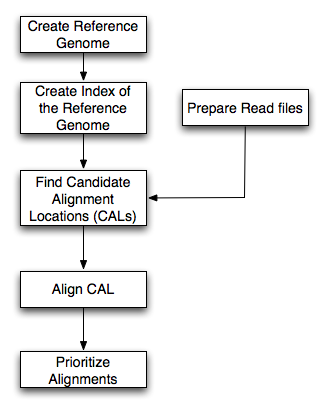
\includegraphics[scale=0.45]{figures/workflow.png} 
%
%\caption{\small Overall workflow for a mapping procedure using BFAST.  In this work, we focus on the step for finding Candidate Alignment Locations (CALs).  }
%  \label{fig:workflow-bfast} 
% \end{figure}
%
%
%\begin{table}
%\begin{tabular}{|c|c|c|c|} 
%  \hline 
% BFAST command & Description & Features for \\ 
%  &  &     Parallelism \\ \hline \hline
%\texttt{bfast fasta2brg} & creation of a ref. genome  &    multiple independent contigs \\ \hline 
%\texttt{solid2fastq}  &  preparation of short reads files &     multiple sequence reads files \\ \hline
%
%\texttt{bfast index} & creation of reference genome indexes& multi-threading and  \\
% &   & low memory option  \\  \hline
%\texttt{bfast match} & finding candidate alignment locations  &  multi-threading and  \\
%& &  parallel execution \\ \hline
%\texttt{bfast localalign} & alignment of each CAL  &   parallel execution \\  \hline
%\texttt{bfast postprocess} & prioritization of alignments  &  parallel execution \\ \hline
%
%
%\hline
%\end{tabular} \caption{Description of BFAST commands and features for parallel and multi-threading execution}
% \label{table:bfast-summary} 
%\end{table}
%

\subsection{TeraGrid Usage by the life science community}

The single largest community is the life-sciences community --
including MD (25\%)...
Get a break-down of the total usage of the TG by discipline and
application type.

\section{Four types of LifeScience Applications}

\subsection{one subsection for each application}

\subsection{Derive what the computational requirements and challenges
  for these applications are}


\jhanote{At the end we propose DARE based Gateways as a solution}


\section{Distributed Adaptive Runtime Environment}

\subsection{SAGA and BigJob abstraction}

To execute a scientific application using heterogeneous distributed computing resources, we develop the Distributed Adaptive Runtime Environment (DARE) framework\cite{dareurl}.  The framework is compose of an open source Web application framework, Pylons
and middleware of the application management system built upon SAGA an BigJob abstraction\cite{saga-ccgrid10,saga-royalsoc,saga-web,jha2009developing,ecmls10}.  This combination of the open source technology and the application management system enables us to develop a lightweight, extensible, full-fledged distributed computing science gateway quickly and effectively\cite{pylonsurl}. 

\subsection{Architecture}

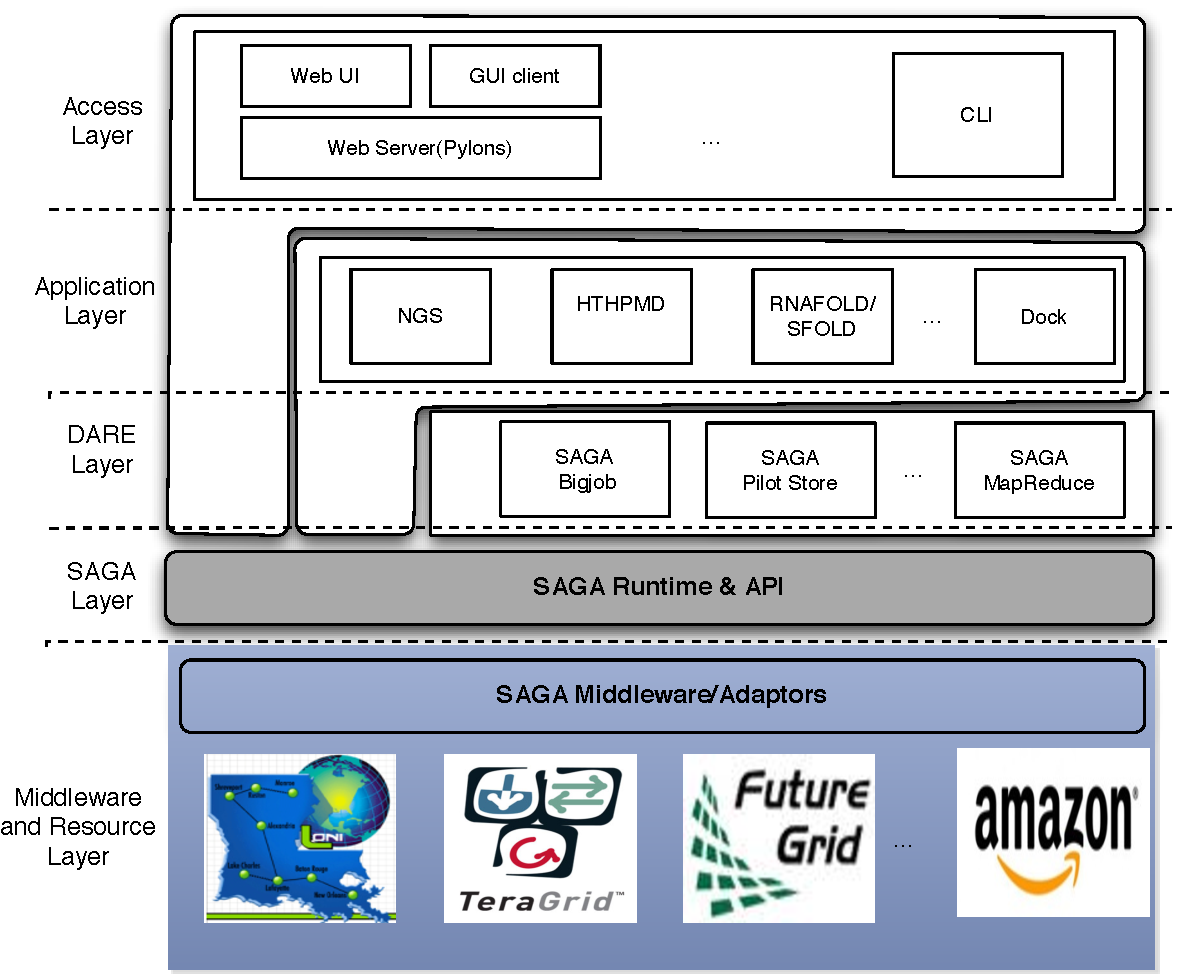
\includegraphics[scale=0.70]{figures/DAREOutline.pdf}

\subsection{The three components -- Access Layer, Services Layer and
  Resource/Provisioning Layer} 

Level 2: (i) Computational aspect, (ii) Data managment and movement, 

Level 1: (iii)providing user interface

\section{three DARE-based Gateways}

\subsection{How does this meet the requirements}
\smnote{ 1) Lets say we have "n" read files and with DARE it takes around time "t" time for matching step if we run it serially it would take n*t time. It probably exceeds wall time limit. Therefore speed up in match step depends how many number of read files we generate and process concurrently.
2) Yes we were able to process the complete run with entire Human Genome on QB and Ranger separately. (**I am currently working this to utilizing QB and Ranger together.) 
4) it should clearly provide the advantage with multiple resources. If we want to use the cloud resources from India to complete Human Genome run it is not practically possible because of the current limited disk size access provided by the FG Eucalyptus resources. Because whole human genome index files are of size 129 GB for Bfast matching step as opposed to HG 18 Chromosome 21 with size of  2 GB index files. On the other hand it also requires the temporary files disk space.  Thus it is important to utilize large capacity resources like QB and Ranger divide the work load across machines.}


\bibliographystyle{abbrv}
\bibliography{tg11}




\end{document}

